\section*{\color{olive}Ejercicio 1: Medici\'on de curvas caracter\'isticas de diodos}

\begin{figure}[h!]
 \begin{center}
    \begin{circuitikz}
    \draw (0,3)
	%(0,0) node[ground] {}
      to[V,v=$V_{cc}$] (0,0) % The voltage source
	(0,3) to[Do] (2,3)
%  (0,3) to[short] (1,3) node[fulldiodeshape]{} 
%	(1,3) to[short] (2,3)
      to[R=$R_1$] (2,0) % The resistor
	to[short] (2,0)
	to[short] (1,0) node[ground]{}
	(1,0) to[short] (0,0);

    \draw (6,3)
	%(0,0) node[ground] {}
      to[V,v=$V_{cc}$] (6,0) % The voltage source
	(6,3) to[zDo] (8,3)
%  (0,3) to[short] (1,3) node[fulldiodeshape]{} 
%	(1,3) to[short] (2,3)
      to[R=$R_1$] (8,0) % The resistor
	to[short] (8,0)
	to[short] (7,0) node[ground]{}
	(7,0) to[short] (6,0);

    \draw (12,3)
	%(0,0) node[ground] {}
      to[V,v=$V_{cc}$] (12,0) % The voltage source
	(12,3) to[leDo] (14,3)
%  (0,3) to[short] (1,3) node[fulldiodeshape]{} 
%	(1,3) to[short] (2,3)
      to[R=$R_1$] (14,0) % The resistor
	to[short] (14,0)
	to[short] (13,0) node[ground]{}
	(14,0) to[short] (12,0);
    \end{circuitikz}

    \caption{\color{cyan}Circuitos empleados para medir la curva caracter\'istica de un diodo rectificador, de un diodo zener y de un LED; respectivamente.}
\end{center}
\end{figure}

%%% diodo rectificador
\subsection*{\color{orange}Diodo rectificador}

A continuaci\'on se presentan los gr\'aficos de la corriente vs. tensi\'on para el caso del diodo rectificador 1N4148. 

\begin{figure}[!ht]
\centering
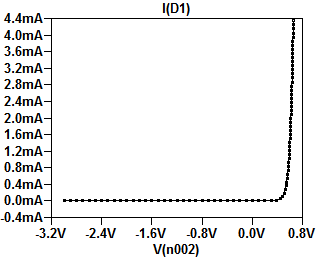
\includegraphics[scale=0.62]{../EJ1/DiodoRectificador/corrienteDiodo1}
%\caption{Simulaci\'on corriente vs. tensi\'on del diodo rectificador.}
%\label{med1a}
%\end{figure}
%\hspace{0.5cm}
%\begin{figure}[!ht]
%\centering
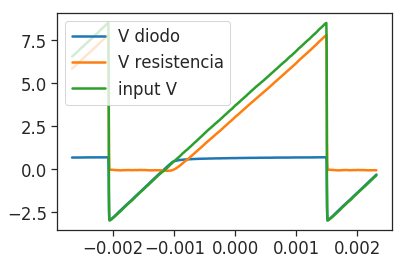
\includegraphics[scale=0.45]{../EJ1/DiodoRectificador/datosOsciloscopio}
%\caption{Medici\'on corriente vs. tensi\'on del diodo rectificador.}
%\label{med1b}
%\end{figure}
%\hspace{0.5cm}
%\begin{figure}[!ht]
%\centering
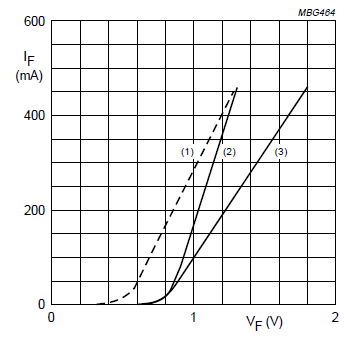
\includegraphics[scale=0.52]{../EJ1/DiodoRectificador/corrienteDiodoDatasheet}

\caption{Corriente vs. tensi\'on del diodo rectificador simulada, medida y obtenida de la hoja de datos; respectivamente.}
\label{med1c}
\end{figure}


%%% diodo zener
\subsection*{\color{orange}Diodo zener}

\begin{figure}[!ht]
\centering
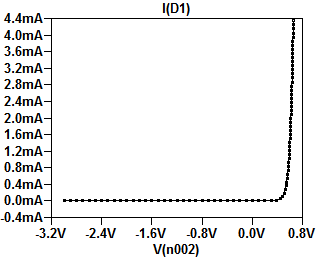
\includegraphics[scale=0.45]{../EJ1/DiodoRectificador/corrienteDiodo1}
\caption{Simulaci\'on corriente vs. tensi\'on del diodo rectificador.}
\label{med2a}
\end{figure}

\begin{figure}[!ht]
\centering
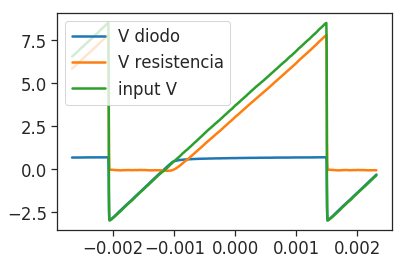
\includegraphics[scale=0.45]{../EJ1/DiodoRectificador/datosOsciloscopio}
\caption{Medici\'on corriente vs. tensi\'on del diodo rectificador.}
\label{med2b}
\end{figure}

\begin{figure}[!ht]
\centering
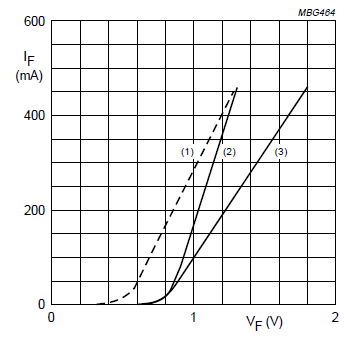
\includegraphics[scale=0.45]{../EJ1/DiodoRectificador/corrienteDiodoDatasheet}
\caption{Corriente vs. tensi\'on del diodo rectificador 1N4148, obtenido de la hoja de datos.}
\label{med2c}
\end{figure}

%%% led
\subsection*{\color{orange}LED}

\begin{figure}[!ht]
\centering
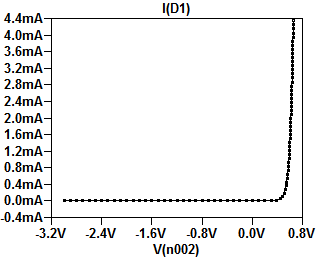
\includegraphics[scale=0.45]{../EJ1/DiodoRectificador/corrienteDiodo1}
\caption{Simulaci\'on corriente vs. tensi\'on del diodo rectificador.}
\label{med3a}
\end{figure}

\begin{figure}[!ht]
\centering
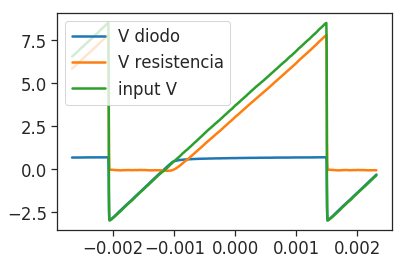
\includegraphics[scale=0.45]{../EJ1/DiodoRectificador/datosOsciloscopio}
\caption{Medici\'on corriente vs. tensi\'on del diodo rectificador.}
\label{med3b}
\end{figure}

\begin{figure}[!ht]
\centering
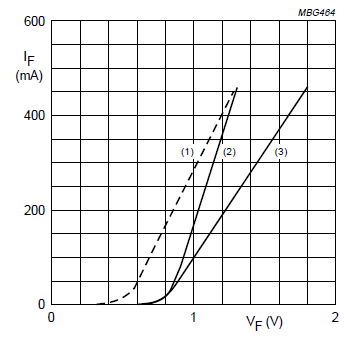
\includegraphics[scale=0.45]{../EJ1/DiodoRectificador/corrienteDiodoDatasheet}
\caption{Corriente vs. tensi\'on del diodo rectificador 1N4148, obtenido de la hoja de datos.}
\label{med3c}
\end{figure}
